\section{Evaluation}

\subsection{Evaluating Results}
\label{subsec:Evaluating Results}

\noindent
Model performance was assessed using the metrics defined in the Phase 4 test design. The table below presents the evaluation results for all three models on the held-out test set.

\begin{table}[ht]
\centering
\small
\begin{adjustbox}{max width=\textwidth}
\begin{tabular}{|l|r|r|r|r|r|r|r|}
\hline
\hline
Model & MAE & MSE & RMSE & R\textsuperscript{2} & ASE & SSE & ObservedAvg\\
\hline
Random Forest & 35.58 & 5978.4 & 77.32 & 0.946 & 5978.4 & 169913246.5 & 1016.17\\
HistGradientBoosting & 47.07 & 7344.9 & 85.70 & 0.934 & 7344.9 & 208749725.6 & 1016.17\\
XGBoost & 46.47 & 6820.1 & 82.58 & 0.939 & 6820.1 & 193833558.3 & 1016.17\\
\hline
\hline
\end{tabular}
\end{adjustbox}
\caption{Model Performance Metrics Comparison}
\label{tab:model_performance}
\end{table}

\vspace{-24pt}
\noindent
The metrics in Table \ref{tab:model_performance} serve distinct purposes in evaluating rental price predictions. MAE values range from \$35.58 (Random Forest) to \$47.07 (HistGradientBoosting), reporting the average absolute dollar error — the most interpretable metric for a business audience. MSE and SSE reflect squared errors and penalise large mistakes more heavily; the large SSE values (e.g., 170M for Random Forest) are expected given 28,421 test records and do not indicate poor fit — they are dataset-size-dependent. RMSE values range from \$77.32 to \$85.70, bringing squared error back to dollar units for direct model comparison. R\textsuperscript{2} (0.934--0.946) measures the proportion of variance in price explained by the model and is scale-independent: a value of 0.946 means the model accounts for 94.6\% of the price variation in the test set, leaving only 5.4\% unexplained. This is strong for housing data, where factors like lease terms, property condition, and negotiation outcomes are not captured.

\noindent
Random Forest achieved the highest R\textsuperscript{2} of 0.946 and the lowest error metrics across all categories, indicating the strongest predictive performance among the three models. XGBoost ranked second with an R\textsuperscript{2} of 0.939, while HistGradientBoostingRegressor achieved an R\textsuperscript{2} of 0.934. All three models performed well, with the gap between the best and worst model being only 0.012 in R\textsuperscript{2}. The R\textsuperscript{2} values across all three models are tightly clustered (range 0.934--0.946), which means the choice of tree-based ensemble matters less than the feature engineering decisions that all three models share -- particularly location clustering.

\noindent
For this project, these results mean that Random Forest is the strongest candidate for estimating rental prices from listing data. Its performance suggests that the model can produce predictions reasonably close to actual prices for many properties in the dataset, making it the most reliable of the three tested approaches. The Observed Average price of \$1,016.17 provides a meaningful baseline: Random Forest's MAE of \$35.58 represents an average prediction error of approximately 3.5\% relative to the mean listing price, which is a strong result for this domain. This is important because the main goal of the project is to produce a predictive understanding of what drives apartment listing prices in the Southern United States.

\noindent
The feature importance results confirm that location-based features are the dominant drivers of rental price. The location\_cluster feature created by K-Means clustering ranked as the most important predictor across all three models (see Table~\ref{tab:fi_ranking} in Phase~4 for the full ranking). Region and square footage (sqfeet) consistently appeared in the top three across all models.

\noindent
The cross-model agreement is notable: location\_cluster is the most important predictor in every model, confirming that geographic clustering captured meaningful price variation that individual region labels alone could not. For renters, this means the model can help assess whether a property is reasonably priced relative to its area and size. For landlords and property managers, it shows which factors have the greatest influence on expected rental value, and that individual amenities such as laundry options or pet policies matter far less than location and size.

\begin{figure}[h!]
    \centering
    \caption{Observed vs Predicted Values}
    \label{fig:OvP}

    \begin{subfigure}[b]{0.329\textwidth}
        \centering
        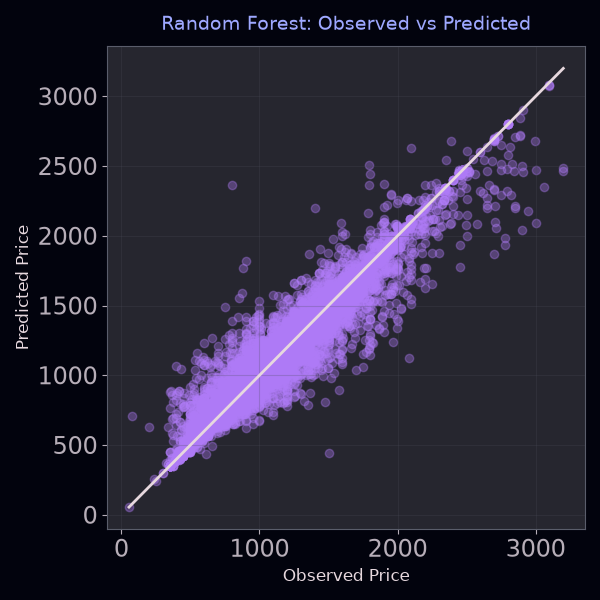
\includegraphics[width=\textwidth]{Assignment/Phase1-5_new/charts/Random Forest: Observed vs Predicted.png}
        \caption{Random Forest}
        \label{fig:OvP_RF}
    \end{subfigure}
    \hfill
    \begin{subfigure}[b]{0.329\textwidth}
        \centering
        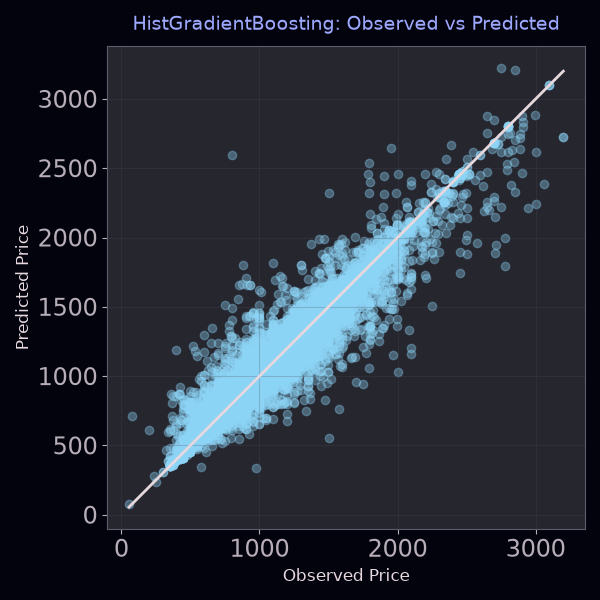
\includegraphics[width=\textwidth]{Assignment/Phase1-5_new/charts/HistGradientBoosting: Observed vs Predicted.png}
        \caption{HistGradientBoosting}
        \label{fig:OvP_GB}
    \end{subfigure}
    \hfill
    \begin{subfigure}[b]{0.329\textwidth}
        \centering
        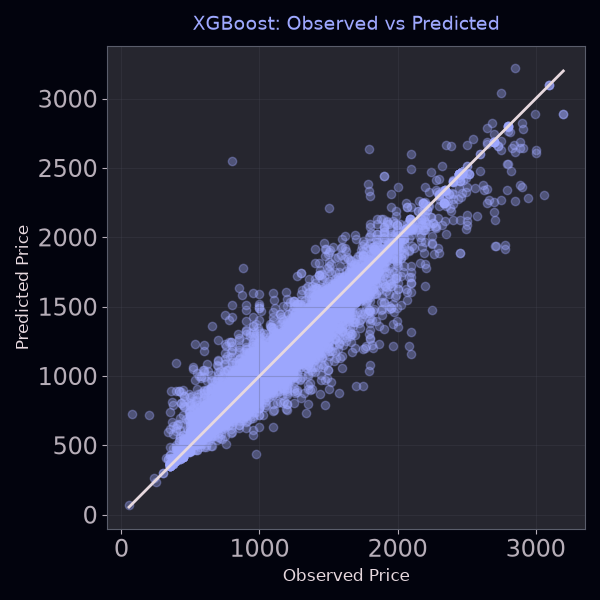
\includegraphics[width=\textwidth]{Assignment/Phase1-5_new/charts/XGBoost: Observed vs Predicted.png}
        \caption{XGBoost}
        \label{fig:OvP_XGB}
    \end{subfigure}
\end{figure}

\noindent
The observed-versus-predicted plots (Figure \ref{fig:OvP}) further support the usefulness of the modeling approach, since most predictions follow the general trend of the actual values. However, a slight broadening of the spread at higher price levels suggests that the models are less precise for the most expensive listings. This indicates the project shows strong promise, but is not yet ready for deployment without further tuning and validation.

\subsection{Reviewing the Process}

\noindent
The process review captures several important lessons from the project, organized by what worked well, what did not work as expected, and what could be done differently in future iterations.

\subsubsection{What Worked Well}
\noindent
The CRISP-DM framework provided effective structure for moving from business objectives through data preparation and modeling. The decision to apply all preprocessing (target encoding, K-Means clustering) inside a pipeline fitted only on the training partition prevented data leakage and ensured that test metrics were honest.

\noindent
Region-sensitive IQR outlier handling was a clear improvement over national-level filtering. By treating each region's price distribution independently, the models avoided discarding valid high-end listings from expensive markets while still removing true outliers in cheaper areas. The improvement was visible in both R\textsuperscript{2} and MAE after the switch.

\subsubsection{What Did Not Work}
\noindent
Individual amenity features (pet policies, smoking, wheelchair access, EV charging, furnished) showed limited predictive power despite being the project's primary analytical focus. The models consistently ranked location and size far above any amenity flag.
\vspace{-12pt}
\begin{itemize}[itemsep=-9pt]
    \item \textbf{What might be tried differently:} Amenity interactions (e.g., ``luxury bundle'' combining in-unit laundry, parking, and pet-friendliness) or relative price premiums (amenity present / amenity absent) could reveal effects that individual binary flags miss. The binary flags alone do not capture price interactions effectively.
    \item \textbf{What this means going forward:} While the project successfully ranked amenity importance, it is possible that Craigslist amenity data is too sparse or inconsistently reported to draw strong conclusions about individual amenities. Future work should consider supplementary data sources.
\end{itemize}

\noindent
The models showed reduced precision at higher price levels (broadening of the observed-vs-predicted spread). This limitation is inherent to the dataset: high-end listings are fewer and their price determinants may differ from the general market. If accurate prediction of luxury rentals were a priority, a separate model trained exclusively on that segment would be appropriate.

\subsubsection{What Would Be Done Differently}
\vspace{-12pt}
\begin{itemize}[itemsep=-9pt]
    \item \textbf{Earlier feature engineering experimentation:} Location clustering was added relatively late in the modeling phase. Starting with a richer feature set earlier would have allowed more iterations.
    \item \textbf{Systematic hyperparameter tuning:} Parameter tuning was done manually (e.g., increasing n\_estimators from 200 to 500, max\_depth from 6 to 7). A grid search or Bayesian optimization would have produced more defensible parameter choices.
    \item \textbf{Structured error analysis:} Instead of evaluating metrics globally, a breakdown by region, price tier, and amenity count would reveal where the model fails systematically.
    \item \textbf{More rigorous data collection documentation:} Recording exactly which features were available at each stage of cleaning would have simplified traceability.
\end{itemize}

\subsection{Determining the Next Steps}

\noindent
The following potential improvements were identified for future iterations of this project:

\vspace{-12pt}
\begin{itemize}[itemsep=-9pt]
    \item Optimize K-Means clustering by systematically finding the optimal number of clusters (e.g., elbow method or silhouette scores) rather than matching the number of Craigslist regions.
    \item Using newer and larger datasets would improve model relevancy to current market forces and expand geographic coverage beyond the Southern USA.
    \item Use GPU/CUDA acceleration (requiring hardware upgrade from the current 2 vCPU/2 GB RAM environment) to speed up training, tuning, and hyperparameter search for more extensive experimentation.
    \item Combining all three models in a weighted ensemble could improve prediction reliability by leveraging the strengths of each approach.
    \item Additional feature engineering (such as price-per-square-foot ratios, proximity to urban centers, or property age estimation) could capture further explanatory power.
    \item In a future iteration with expanded hardware and tooling, NLP analysis of the \texttt{description} field could reveal insights missed by structured features, such as renovation quality or neighborhood character.
\end{itemize}

\vspace{-9pt}

\noindent
On average, all three models performed well, and the modeling approach showed promising predictive performance. However, the project is not yet ready for deployment as-is. The final recommendation is to revise and improve the work before deployment, since the results are encouraging but further tuning, extension, and validation are still needed.

\vspace{150pt}
\textcolor{white}{.}
